\section{Questão 140 - Notação Científica}

A gripe é uma infecção respiratória aguda de curta duração causada pelo vírus influenza. Ao entrar no nosso organismo pelo nariz, esse vírus multiplica-se, disseminando-se para a garganta e demais partes das vias respiratórias, incluindo os pulmões. 

O vírus influenza é uma partícula esférica que tem um diâmetro interno de 0,00011 mm.

\begin{flushright}
    {\scriptsize Disponível em: www.gripenet.pt. Acesso em: 2 nov. 2013 (adaptado).}
\end{flushright}

Em notação científica, o diâmetro interno do vírus influenza, em mm, é

(A)  $ 1,1 \times 10^{-1} $

(B)  $ 1,1 \times 10^{-2} $

(C)  $ 1,1 \times 10`{-3} $

(D)  $ 1,1 \times 10^{-4} $

(E)  $ 1,1 \times 10^{-5} $

\textbf{Resolução}

Um número na notação científica é um número na forma $ N \times 10^{n} $ onde N é o primeiro dígito significativo entre 1 e 10 e n é a quantidade de zeros a direita (negativo) ou a esquerda (positivo) do número, ou matematicamente $ N \times 10^{n} $ | $1 \leqslant N < 10 $ e $n \in \mathbbm{Z} $

\tikzset{every picture/.style={line width=0.75pt}} %set default line width to 0.75pt        

\noindent \resizebox{.5\textwidth}{!}{

    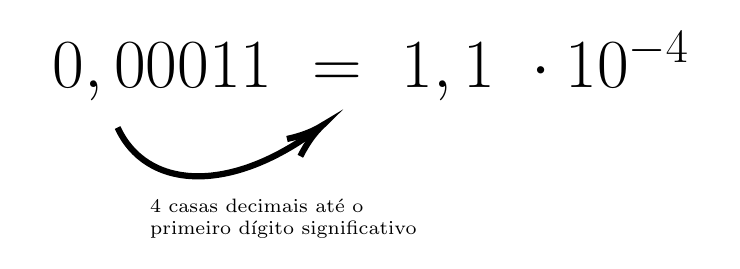
\begin{tikzpicture}[x=0.75pt,y=0.75pt,yscale=-1,xscale=1]
    %uncomment if require: \path (0,139); %set diagram left start at 0, and has height of 139
    
    %Curve Lines [id:da5246758628503831] 
    \draw [line width=2.25]    (66.83,66) .. controls (80.23,95.4) and (119.87,98.87) .. (162.86,67) ;
    \draw [shift={(165.5,65)}, rotate = 502.31] [color={rgb, 255:red, 0; green, 0; blue, 0 }  ][line width=2.25]    (17.49,-5.26) .. controls (11.12,-2.23) and (5.29,-0.48) .. (0,0) .. controls (5.29,0.48) and (11.12,2.23) .. (17.49,5.26)   ;
    
    % Text Node
    \draw (24,18.4) node [anchor=north west][inner sep=0.75pt]  [font=\fontsize{2.59em}{3.11em}\selectfont]  {$\ 0,00011\ =\ 1,1\ \cdot 10^{-4} \ $};
    % Text Node
    \draw (81,99) node [anchor=north west][inner sep=0.75pt]  [font=\scriptsize] [align=left] {4 casas decimais até o \\primeiro dígito significativo};
    
    
    \end{tikzpicture}


}


\begin{center}
    \href{https://youtu.be/hRFaaCCGBQo}{
        \qrcode{https://youtu.be/hRFaaCCGBQo}
    }\\
    {\scriptsize Resolução: \url{https://youtu.be/hRFaaCCGBQo}}
\end{center}